% Drawing 136/02-1 -- folder 136, batch 02, archive page 36 (PDF page 37).
% Transcription: une boucle et quelques points, avec des flèches à double pointe partant d'un sommet, étiquetées $x$ et $xg$ ; au-dessous « Diagramme de Cayley » et un encadré « $g$, $g'$, $gh$ » ; une seconde boucle et deux flèches horizontales vers la gauche.
% Kind: Cayley diagram sketch: loop, points, double-headed arrows. Method 2 (schematic redraw from the facsimile). Status: ok.
% Notes: The lower half of p. 36 is written upside down; crop rotated 180 degrees and redrawn upright on a tight crop. The box (now drawn) with its contents kept as the transcription reads them, g, g', gh (on the crop they read like g, g_1, ..., g_k); two horizontal arrows to its right, the first with a single head in its middle, the second with a double head (>>) near its start; "Diagramme de Cayley". The loop starts and ends at a vertex, passing through a second vertex above it; the arrows are double-pointed in the sense of two chevrons (>>), not heads at both ends as drawn before: from the upper vertex to the right, and from the lower vertex along the straight stroke xg to its point, and down to the right (x); a short tail down to the left. Points: the vertex, the end of xg, two at the far left, a row of three to the right; the second loop on the right ends at g. Left out: the three long oblique strokes crossing the region (read as strikes; drawn grey before), the upside-down sentence at the bottom (text), the typed text showing through. Still a reading: the box contents and the double heads (rendered with two Stealth tips). Redrawn 2026-11-09 (issue 128): to check again. Question settled by a machine pass on the facsimile, 2026-11-12 (page): the arrows carry double chevrons (>>) along the stroke, as the legend of two arrows beside the box shows (one with a single head, one with a double head); drawn so already. Not checked by a reader. Question settled by a machine pass on the facsimile, 2026-11-12 (page): the box reads G, g_1, [gap], g_k (a large first letter, then indexed g's; the line « Mot en les g_i + origine » under the figure has the same g_i), not g, g', gh; the label is corrected, with the gap left as on the page; the transcription's reading is to be corrected there. Not checked by a reader. Question settled by a machine pass on the facsimile, 2026-11-12 (page): the three long oblique strokes run far beyond the figure, across the box corner, the caption and the lines below: they cancel this part of the sheet and are not part of the Cayley diagram; they stay left out. Not checked by a reader. 2026-11-13, Claude Opus 5.5, overlay check (issue 147): not compiled (no TeX in the session); the TikZ rasterised and laid over the 259 ppi colour scan (rendered at 350 dpi, crop turned 180 degrees). Changed: the loop redrawn through points read on its ink (its right end was up to 0.7 unit off); the heavy dot of the upper vertex added; the second, inner stroke between the two vertices added, with the arrowhead pointing up that stands between it and the loop (drawn on the inner stroke: on the page it straddles both); the double chevrons placed where they stand (mid-stroke on the upper arrow, near the start of xg, near the end of x), and the second legend arrow's two chevrons at 61.4 and 63; the small dot at (62.7, 39) and the short thin tail of the dot left of g added; the labels x, xg, g moved onto their ink; the second loop redrawn through its ink. Every element now lies on the ink to within about 0.5 unit. Left out as before: the three long oblique strokes that cancel this part of the sheet, the upside-down sentence, the typed text showing through, and a faint grey stroke with specks below the two left points (about (7, 54) to (14.5, 48.5)), which reads as show-through, not as ink of the figure.
% Coordinates: 1 unit = 1 mm = 1/100 of the crop width (bbox in page fractions: [0.15, 0.52, 0.85, 0.87]).
% Redrawn by Claude (claude-opus-5-5), issue #73, 2026-11-09; not checked by a human; not compiled (no TeX in the session).
% Revised by Claude Opus 5.5 (claude-opus-5-5), issue #147, 2026-11-13: overlay check on the colour scan; not checked by a human; not compiled (no TeX in the session).
% Rights: reproduces part of the work -- behind RENDER_TRANSCRIPTS, never published by itself.
\documentclass[tikz,border=3pt]{standalone}
\usepackage{amsmath,amssymb}
\usetikzlibrary{patterns,arrows.meta}
\tikzset{pencil/.style={black!45}, struck/.style={black!35}, mark/.style={circle,draw,inner sep=1.3pt}, pt/.style={circle,fill,inner sep=0.9pt}, opt/.style={circle,draw,fill=white,inner sep=1.1pt}}
\begin{document}
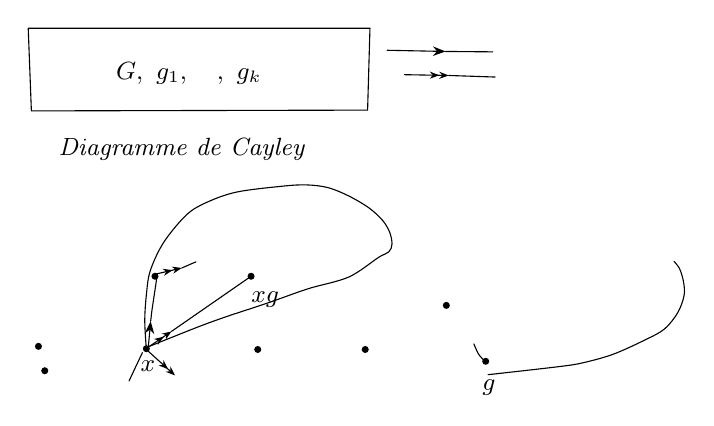
\begin{tikzpicture}[x=1mm,y=1mm,line cap=round,line join=round,font=\scriptsize]
\draw (9.6,-3.8) -- (53,-3.8) -- (52.7,-14.2) -- (10,-14.3) -- cycle;
\node[inner sep=1pt] at (30,-9.6) {\small $G,\ g_1,\quad,\ g_k$};
\draw[-{Stealth[length=1.6mm]}] (55.2,-6.6) -- (62.6,-6.75);
\draw (62.6,-6.75) -- (68.6,-6.8);
\draw[-{Stealth[length=1.2mm]Stealth[length=1.2mm]}] (57.4,-9.7) -- (63,-9.8);
\draw (63,-9.8) -- (68.9,-10);
\node[inner sep=1pt] at (29.2,-19.2) {\small \textit{Diagramme de Cayley}};
\draw plot[smooth, tension=0.55] coordinates {(24.6,-44.5) (24.4,-41) (24.6,-37.7) (25.1,-34.6) (26.8,-31) (29.7,-27.5) (32.3,-25.9) (36.1,-24.6) (42,-23.85) (45,-23.7) (47.7,-24.05) (50.3,-25.1) (52.85,-26.6) (54.6,-28.2) (55.5,-29.7) (55.8,-31.2) (55.4,-32.2) (54.1,-32.9) (50.3,-35.4) (45.1,-36.9) (40,-38.7) (34.85,-40.4) (31,-41.8) (25,-44.2)};
\draw[-{Stealth[length=1.6mm]}] (24.85,-44.3) -- (25.15,-41);
\draw (25.15,-41) -- (25.3,-39.7) -- (25.9,-35.7);
\draw[-{Stealth[length=1.2mm]Stealth[length=1.2mm]}] (25.9,-35) -- (29.1,-34.25);
\draw (29.1,-34.25) -- (30.9,-33.47);
\draw[-{Stealth[length=1.2mm]Stealth[length=1.2mm]}] (25,-44.2) -- (27.8,-42.3);
\draw (27.8,-42.3) -- (37.9,-35.3);
\node[inner sep=1pt] at (39.7,-38.2) {\small $xg$};
\draw[-{Stealth[length=1.2mm]Stealth[length=1.2mm]}] (24.6,-44.6) -- (28.25,-47.9);
\node[inner sep=1pt] at (24.8,-46.7) {\small $x$};
\draw (24.1,-45) -- (22.4,-48.6);
\node[pt] at (24.6,-44.5) {};
\node[pt] at (25.7,-35.3) {};
\node[pt] at (37.9,-35.3) {};
\node[pt] at (10.9,-44.2) {};
\node[pt] at (11.7,-47.3) {};
\node[pt] at (38.75,-44.6) {};
\node[pt] at (52.4,-44.6) {};
\node[pt] at (62.7,-39) {};
\draw plot[smooth, tension=0.55] coordinates {(66.2,-43.9) (66.8,-45.2) (67.6,-46.1)};
\node[pt] at (67.7,-46.1) {};
\draw plot[smooth, tension=0.55] coordinates {(68,-47.8) (76.8,-46.8) (80,-46.3) (83.9,-45.2) (87.9,-43.4) (90.4,-42) (92.1,-39.9) (92.9,-37.7) (92.8,-35.9) (92.3,-34.3) (91.6,-33.4)};
\node[inner sep=1pt] at (68.1,-49.4) {\small $g$};
\end{tikzpicture}
\end{document}
